%                                             -*- coding: utf-8 -*-
% Using LaTeX is highly recommended. 
% If you correct/upgrade anything please send it back to help others' work.

\documentclass[a4paper,oneside]{article}
\usepackage[margin=3cm]{geometry}
% =================================================================
\usepackage[english]{babel}
\selectlanguage{english}

%=================================================================
% Font encoding
% The T1 font encoding is an 8-bit encoding and uses fonts that have 256 glyphs.
\usepackage[T1]{fontenc}
\usepackage[utf8]{inputenc}
\usepackage{multirow} 
%================================================================
% Use Times New Roman
\usepackage{times}

%================================================================
% Figures
% usage: \includegraphics[width=<width>]{fig.png}
\usepackage{graphicx}
\usepackage{wrapfig}

%================================================================
% Citations
\usepackage{natbib}

% images root folder
\graphicspath{{./figs/}}

%================================================================
% Package to create pdf hyperlinks
%------------------------------------
% Hyperref should be the last imported (except some problematic packages, e.g. algorithm)
\usepackage[colorlinks=true]{hyperref}


%%%%%%%%%%%%%%%%%%%%%%%%%%%%%%%%%%%%%%%%%%%%%%%%%%%%%%%%%%%%%%%%%%%
% HERE IS THE START OF THE DOCUMENT
%%%%%%%%%%%%%%%%%%%%%%%%%%%%%%%%%%%%%%%%%%%%%%%%%%%%%%%%%%%%%%%%%%
\begin{document}
%%%%%%%%%%%%%%%%%%%%%%%%%%%%%%%%%%%%%%%%%%%%%%%%%%%%%%%%%%%%%%%%%%%
% Do not modify if you don't know what you are doing!!!!
%%%%%%%%%%%%%%%%%%%%%%%%%%%%%%%%%%%%%%%%%%%%%%%%%%%%%%%%%%%%%%%%%%%
\pagestyle{myheadings} % use heading 

\newcommand{\projectlaboratorytitle}{
  \begin{center}
    \huge{\textbf{Project Laboratory Report}}
    
    \smallskip
    \small{Department of Telecommunications and Media Informatics}
  \end{center}
  \bigskip
} 

% #1=Name, #2=Neptun, #3=Specialization, #4=Email, #5 Supervisor-1, #6 Supervisor-1-Email, #7 Supervisor-2, #8 Supervisor-2-Email
\newcommand{\projectlaboratoryauthor}[8]{

\begin{center}
  \begin{tabular}{ l c }
  Author:         & \textbf{#1}  \\
  Neptun:         & \textbf{\texttt{#2}}  \\
  Specialization: & \textbf{#3}  \\
  E-mail address: & \href{mailto:#4}{\textbf{#4}}  \\
  Supervisor:     & \textbf{#5}  \\
  E-mail addres:  & \href{mailto:#6}{\textbf{#6}} \\
  Co-Supervisor:  & \textbf{#7}  \\
  E-mail addres:  & \href{mailto:#8}{\textbf{#8}} \\
  
  \end{tabular}
\end{center}
\bigskip

}

% Arguments: #1=Semester (format: xxxx/xx , #2=I/II (without dot!))
\newcommand{\semester}[2]{
  \large\textbf{#1 #2. semester}
}

% Arguments: #1=Title
\newcommand{\tasktitle}[1]{
  \begin{center}
    \LARGE\textbf{Title: #1}
    \bigskip
  \end{center}
}

% Arguments: #1=Description
\newcommand{\taskdescription}[1]{
\begin{center}
  \Large\textbf{Task} 
\end{center}
#1
\newline
\bigskip
}

% References
% \def\references#1{\renewcommand{%
% \baselinestretch}{1}\list
%  {\small [\arabic{enumi}]}{\settowidth\labelwidth{[#1]}\leftmargin\labelwidth
%  \advance\leftmargin\labelsep
%  \usecounter{enumi}}
%  \def\newblock{\small \hskip .11em plus .33em minus .07em}
%  \sloppy\clubpenalty4000\widowpenalty4000
%  \sfcode`\.=1000\relax}
% \let\endreferences=\endlist%


%%% Local Variables: 
%%% mode: latex
%%% TeX-master: "template"
%%% End: 
 % Import macros
\markright{Szenyán Zsombor (IOA33U)} % one sided title page!!!
%--------------------------------------------------------------------
% title page
%--------------------------------------------------------------------

\begin{titlepage}
%bme logo 
 \begin{figure}[h]
    \centering
      
\includegraphics[width=12cm]{bme_logo.pdf}
  \label{fig:bme_logo}
  \end{figure}
  \thispagestyle{empty}
  
  % generate title
  \projectlaboratorytitle
 
  \projectlaboratoryauthor{Szenyán Zsombor}{IOA33U}{Infocommunication}{zsomborszenyan@edu.bme.hu}{Gyires-Tóth Bálint, PhD}{tothb@tmit.bme.hu}{Kalapos András}{kalapos.andras@edu.bme.hu}
 
 
  %\tasktitle
  \tasktitle{Real-time Facial Attribute Recognition using Transformer networks} 

  %\taskdescription
  \taskdescription{In my project laboratory, I've researched the state-of-the-art solutions in the field of facial attribute recognition and improved on efficiency of existing methods by leveraging Transformer networks.
  By harnessing the power of Transformer architecture, I've constructed a neural network that excels in real-time recognition of facial attributes.
  This new model not only ensures efficient and fast processing but also boasts accuracy levels on par with the current state-of-the-art systems.
  With its ability to swiftly and accurately recognize facial attributes, this project opens doors to real-time applications in various fields, from security systems to personalized user experiences.}

  % semester Arguments: #1=Semester (format: xxxx/xx , #2=I/II (without dot!))
  \begin{center}
    \semester{2023/24}{II}
  \end{center}
  
\end{titlepage} 

%==================================================================
\begin{center}
  \section{Theory and previous works}
  \label{sec:theory_prev}
\end{center}

\subsection{Introduction}
\label{sec:introduction}

Facial attribute recognition, a fundamental task in computer vision, revolves around the identification and analysis of specific facial features and attributes.
These attributes encompass a wide array of characteristics, including but not limited to gender, hair color, and even more nuanced traits like facial hair or glasses.
The ability to accurately recognize these attributes holds significant implications across various domains, ranging from security and surveillance to personalized recommendations and beyond.

In security and surveillance, facial attribute recognition plays a pivotal role in identifying individuals of interest, enhancing the effectiveness of monitoring systems, and aiding law enforcement agencies in their efforts to ensure public safety.
By extracting crucial information from facial attributes, such as distinguishing between authorized personnel and potential threats, these systems contribute to bolstering security measures and preventing security breaches.

In the domain of personalized recommendations, facial attribute recognition can be a useful tool for enhancing user experiences and optimizing content delivery. By discerning users' facial attributes, such as age, gender, and other facial attributes, recommendation systems can tailor their suggestions to align more closely with individual preferences and interests.
For instance, in e-commerce, understanding customers' demographic profiles and emotional states enables platforms to recommend products that resonate with their specific needs and preferences. Whether it's suggesting clothing styles that match a user's age and gender or recommending entertainment content based on their current mood, personalized recommendations powered by facial attribute recognition contribute to enriching the user experience and driving engagement.

Against this backdrop, the aim of this paper is multifaceted. Primarily, it seeks to provide a comprehensive overview of the current state of the art in facial attribute recognition, surveying existing methodologies, techniques, and challenges. Furthermore, the paper aims to explore the potential of leveraging the transformer architecture — a powerful paradigm in natural language processing — in advancing the capabilities of facial attribute recognition systems. By harnessing the transformer's capacity for capturing long-range dependencies and modeling complex relationships, I aspire to enhance the performance, efficiency, and scalability of existing solutions.
Ultimately, the goal is to propel the field towards achieving real-time model performance, thereby unlocking new applications of facial attribute recognition systems.

\subsection{Theoretical summary}
\label{sec:theoretical_summary}

Facial attribute recognition encompasses a diverse set of concepts and methodologies aimed at identifying and analyzing specific facial features and attributes. Key terms and concepts in this field include:

Facial Landmarks: These are specific points on a face, such as the corners of the eyes or the tip of the nose, used to define the geometric structure of the face.

Feature Extraction: This involves the process of extracting meaningful information from facial images, which can include both low-level features like edges and textures and high-level features like facial expressions or facial hair.

Machine Learning Algorithms: Various machine learning algorithms are utilized in facial attribute recognition, including traditional techniques such as Support Vector Machines (SVMs) and decision trees, as well as deep learning models like Convolutional Neural Networks (CNNs) and transformer architectures.

Convolutional Neural Networks (CNNs): CNNs have been pivotal in revolutionizing facial attribute recognition by enabling end-to-end learning of hierarchical features directly from raw image data. They automatically learn and extract features at different levels of abstraction, making them well-suited for tasks like facial attribute classification.

Transformer Architectures: Initially developed for natural language processing tasks, transformer architectures have recently been applied to computer vision tasks, including facial attribute recognition. These architectures excel at capturing long-range dependencies and modeling complex relationships within the data, potentially leading to improved performance in facial attribute recognition tasks.

The theoretical underpinnings of facial attribute recognition often involve the application of deep learning models like CNNs or traditional computer vision techniques. CNNs, with their hierarchical feature extraction capabilities, have become the backbone of many state-of-the-art facial attribute recognition systems. They can automatically learn and extract relevant features from facial images, making them particularly well-suited for tasks like attribute classification.

In recent years, transformer architectures have also gained prominence in facial attribute recognition research. These architectures, originally designed for natural language processing tasks, have shown promise in capturing complex relationships within facial images, potentially leading to improved performance in attribute recognition tasks. The application of transformer architectures represents a theoretical shift towards leveraging attention mechanisms and capturing long-range dependencies within facial images.

Common theoretical frameworks or methodologies used in facial attribute recognition research include:

Deep Learning: Deep learning frameworks, such as CNNs and transformer architectures, are commonly employed due to their ability to automatically learn and extract features from raw data, leading to improved performance in facial attribute recognition tasks.

Multi-Task Learning: This framework involves training a single model to perform multiple tasks simultaneously, such as gender classification, age estimation, and facial expression recognition. By jointly learning from multiple tasks, models can leverage shared representations and potentially improve performance on individual tasks.

Data Augmentation: Data augmentation techniques involve generating additional training samples by applying transformations such as rotation, scaling, or flipping to existing data. This framework helps improve model robustness and generalization by exposing the model to a diverse range of facial variations during training.

Overall, the theoretical landscape of facial attribute recognition is characterized by a combination of traditional computer vision techniques and modern deep learning methodologies, with an increasing emphasis on leveraging advanced architectures like CNNs and transformers to achieve state-of-the-art performance.

\subsection{Starting point, previous works on this project}
\label{sec:prev_works}

In recent years, transformer models have gained prominence in various natural language processing (NLP) tasks and have been increasingly applied to computer vision tasks, including facial attribute recognition. In this section, I review the related work on facial attribute recognition with a specific focus on the application of transformer models.
\subsubsection{Earlier Approaches to Facial Attribute Recognition using Deep Learning}
The advent of deep learning revolutionized facial attribute recognition by enabling end-to-end learning of feature representations directly from raw data. Convolutional Neural Networks (CNNs) emerged as the backbone of many state-of-the-art systems, leveraging their ability to automatically learn hierarchical features.

\citet{DBLP:journals/corr/HandC16} have developed a multi-task deep convolutional neural network (MCNN) for attribute classification.
The proposed architecture, along with an auxiliary network (AUX), significantly improves attribute classification accuracy compared to traditional methods.
Their method achieved state-of-the-art performance on various attributes from the CelebA and LFWA datasets, with some attributes showing up to a 15\% improvement over other methods.
The MCNN architecture significantly reduces the number of parameters and training time required for attribute classification compared to independent CNNs, making it more efficient.
The learned relationships among attributes in the auxiliary network provide insights into the correlations between different attributes, contributing to a better understanding of the underlying data.

\citet{DBLP:journals/corr/GuntherRB16} have demonstrated that the application of data augmentation techniques, including random scaling, rotation, shifting, blurring, and horizontal flipping, not only does not compromise performance but also yields significant benefits.
Their findings underscore the importance of leveraging data augmentation as a powerful strategy to enhance model robustness and performance in various tasks.
By introducing variations in the training data through augmentation, models can learn more generalized features and exhibit improved performance across different scenarios.

\citet{DBLP:journals/corr/HanJSC17} present a novel approach to heterogeneous face attribute estimation using Deep Multi-Task Learning (DMTL) with convolutional neural networks (CNNs).
Unlike previous methods that either focused on estimating a single attribute or used separate models for each attribute without considering attribute correlation and heterogeneity, the proposed DMTL approach addresses these issues explicitly.
The DMTL framework consists of shared feature learning for all attributes followed by category-specific feature learning for heterogeneous attribute categories.
To handle attribute heterogeneity, the paper categorizes attributes into nominal vs. ordinal and holistic vs. local.
Nominal attributes, such as race, are handled using classification schemes with cross-entropy loss, while ordinal attributes, such as age, are handled using regression schemes with Euclidean loss.
Additionally, attributes are categorized as holistic or local based on whether they describe characteristics of the whole face or local facial components, respectively.
The proposed DMTL approach outperforms state-of-the-art methods in face attribute estimation, as demonstrated through experiments on various benchmark datasets.
The approach not only achieves high accuracy but also demonstrates excellent generalization ability, particularly in cross-database testing scenarios.

\subsubsection{Transforming Image Recognition: A Comparative Review of Transformer Networks Versus CNNs}
The transformer architecture, initially proposed for natural language processing (NLP) tasks, has recently been applied to computer vision tasks, including image recognition and object detection,
however the application of transformer models to facial attribute recognition has been relatively limited.
In this section I review the recent work on the application of transformer models to computer vision tasks, with one example of their application in the domain.

One notable approach is the Vision Transformer (ViT) by \citet{DBLP:journals/corr/abs-2010-11929}, which treats image patches as tokens (similar to words in NLP) and processes them using a standard Transformer architecture.
ViT achieves impressive results when pre-trained on large datasets and transferred to various image recognition benchmarks, surpassing state-of-the-art CNN-based models while requiring fewer computational resources.
In contrast to CNNs, ViT exhibits less image-specific inductive bias, with only the MLP layers being local, while the self-attention layers are global.
Positional information is preserved through the addition of learnable position embeddings. 

The Swin Transformer by \citet{DBLP:journals/corr/abs-2103-14030} addresses the challenges of the ViTs by proposing a hierarchical Transformer architecture with shifted windows.
This design enables modeling at various scales while maintaining linear computational complexity with respect to image size, while enhancing modeling power without sacrificing computational efficiency.

It has been demonstrated by \citet{liu2022transfa} that the transformer architecture can be effectively applied to facial attribute recognition tasks.
Inspired by the visualization of feature attention map of different attributes, they naturally group attributes with similar attention regions into the same category.
The proposed TransFa model utilizing the Swin Transformer architecture achieves state-of-the-art performance on the CelebA dataset, outperforming previous methods.

One drawback of the transformer architecture is its computational complexity, which is higher than that of CNNs.
However, \citet{li2022efficientformer} have proposed the EfficientFormer, a lightweight transformer architecture that achieves competitive performance with state-of-the-art CNNs while being more efficient in terms of computational resources.
With an inference time lower than the frametime of most displays or cameras, makes this model suitable for real-time applications.
\citet{li2022rethinking} later introduced the second version of the EfficientFormer, which further improves the performance of the model while maintaining its efficiency.

\subsubsection{Details of the EfficientFormerV2}
% They achieved this by giving the multi-head self attention mechanism (MHSA) an input computed by several local convolutional layers, which allows the model to capture local features more effectively and reducing the number of parameters given to the MHSA.
% Furthermore they improve on the MHSA by downsampling the input and interpolating the output, which allows the model to capture global features more efficiently.
EfficientFormerV2 builds upon the success of previous transformer-based models like Vision Transformers (ViTs) and Swin Transformers but aims to optimize them for efficient deployment on resource-constrained devices, particularly mobile devices.
In this section I break down the improvements and capabilities of EfficientFormerV2 compared to its predecessors.

% Optimization for Mobile Devices
The primary goal of EfficientFormerV2 is to achieve high performance while maintaining a small model size and fast inference speed, crucial for running on mobile devices with limited resources.
The EfficientFormerV2 introduces several architectural improvements to achieve its goals.
It employs a hierarchical design with four stages, capturing both local and global information efficiently.

The architecture starts with a convolutional stem for input embedding, ensuring efficient processing of input images.
% Unified Feed Forward Network (FFN)
Instead of using separate local token mixers, EfficientFormerV2 incorporates depth-wise convolutions into the Feed Forward Network (FFN), reducing redundancy and improving performance with minimal parameter overhead.
% Attention Improvements
EfficientFormerV2 enhances the Multi-Head Self Attention (MHSA) mechanism by injecting local information into the Value matrix and enabling communication between attention heads.
These modifications boost performance without significantly increasing model size or latency.
% Attention on Higher Resolution
To efficiently apply attention to higher-resolution features, EfficientFormerV2 introduces strategies like Stride Attention, which downsamples Queries, Keys, and Values to a fixed spatial resolution.
This approach reduces latency while preserving competitive accuracy.
% Dual-Path Attention Downsampling
EfficientFormerV2 introduces a novel downsampling strategy called dual-path attention downsampling.
This method combines locality and global dependency, improving accuracy without compromising efficiency.

%Joint Optimization
The search algorithm of EfficientFormerV2 considers both model size and inference speed as key factors, aiming to achieve Pareto optimality in terms of Mobile Efficiency Score (MES).
This ensures that the resulting models are efficient for mobile deployment.
With this search algorithm, the authors created 4 models with different trade-offs between model size and inference speed, allowing users to choose the best model for their specific requirements.

Overall, EfficientFormerV2 represents a significant advancement in transformer-based models tailored for mobile deployment.
By combining architectural enhancements, optimization strategies, it achieves higher performance than traditional lightweight CNNs while maintaining small model size and fast inference speed, making it suitable for real-time applications on mobile devices.

\newpage
%==================================================================
\begin{center}
  \section{Own work on project}
  \label{sec:work}
\end{center}

\subsection{Introduction to the dataset}
\label{sec:subsection_dataset_intro}

In this section, I provide an overview of the dataset used to train my facial attribution recognition model.
The CelebA dataset serves as the foundation for our model's training, validation, and testing phases.
With a vast collection exceeding 200,000 images divided into training, validation, and test subsets, CelebA offers a robust platform for evaluating model performance and facilitating comparative analyses with other state-of-the-art approaches.

Each image within the CelebA dataset is standardized to a resolution of 218 by 178 pixels, ensuring consistency across the entire corpus.
Notably, every image is labeled with 40 distinct facial attributes, providing rich annotations needed for supervised learning paradigms.
It should be noted that the dataset's attributes are binary, with each attribute denoting the presence or absence of a specific facial feature or characteristic.
% Attribute imbalance
Furthermore the attributes are not uniformly distributed, with some attributes being more prevalent than others.
This imbalance poses a challenge for training models that must account for the varying frequencies of different attributes.

This comprehensive labeling scheme enables the development and refinement of highly accurate facial attribute recognition models, thereby enhancing the dataset's suitability for various machine learning applications.

\subsection{Dataset preprocessing and augmentation}
\label{sec:subsection_dataset_preprocessing}


Preprocessing plays a crucial role in preparing the dataset for effective model training, while augmentation techniques further enhance the robustness and generalization capability of the trained model, essentially artificially inflating the size of the dataset. In this section, I detail the preprocessing and augmentation steps employed in my approach.

In regards to preprocessing, the following steps were undertaken:

Image Cropping to ensure compatibility with the transformer backbone, each image in the dataset underwent cropping.
Initially sized at 218 by 178 pixels, the images were cropped to form perfect squares of 178 by 178 pixels.
This transformation not only standardizes the input dimensions but also centers the facial features within the frame, facilitating more focused learning.
RGB to Float32 Conversion for quicker gradient descent. The color information encoded in the RGB (Red, Green, Blue) format using 8 bit floating point numbers was converted into floating-point values scaled between 0 and 1.

\begin{wrapfigure}{r}{0.5\textwidth}
  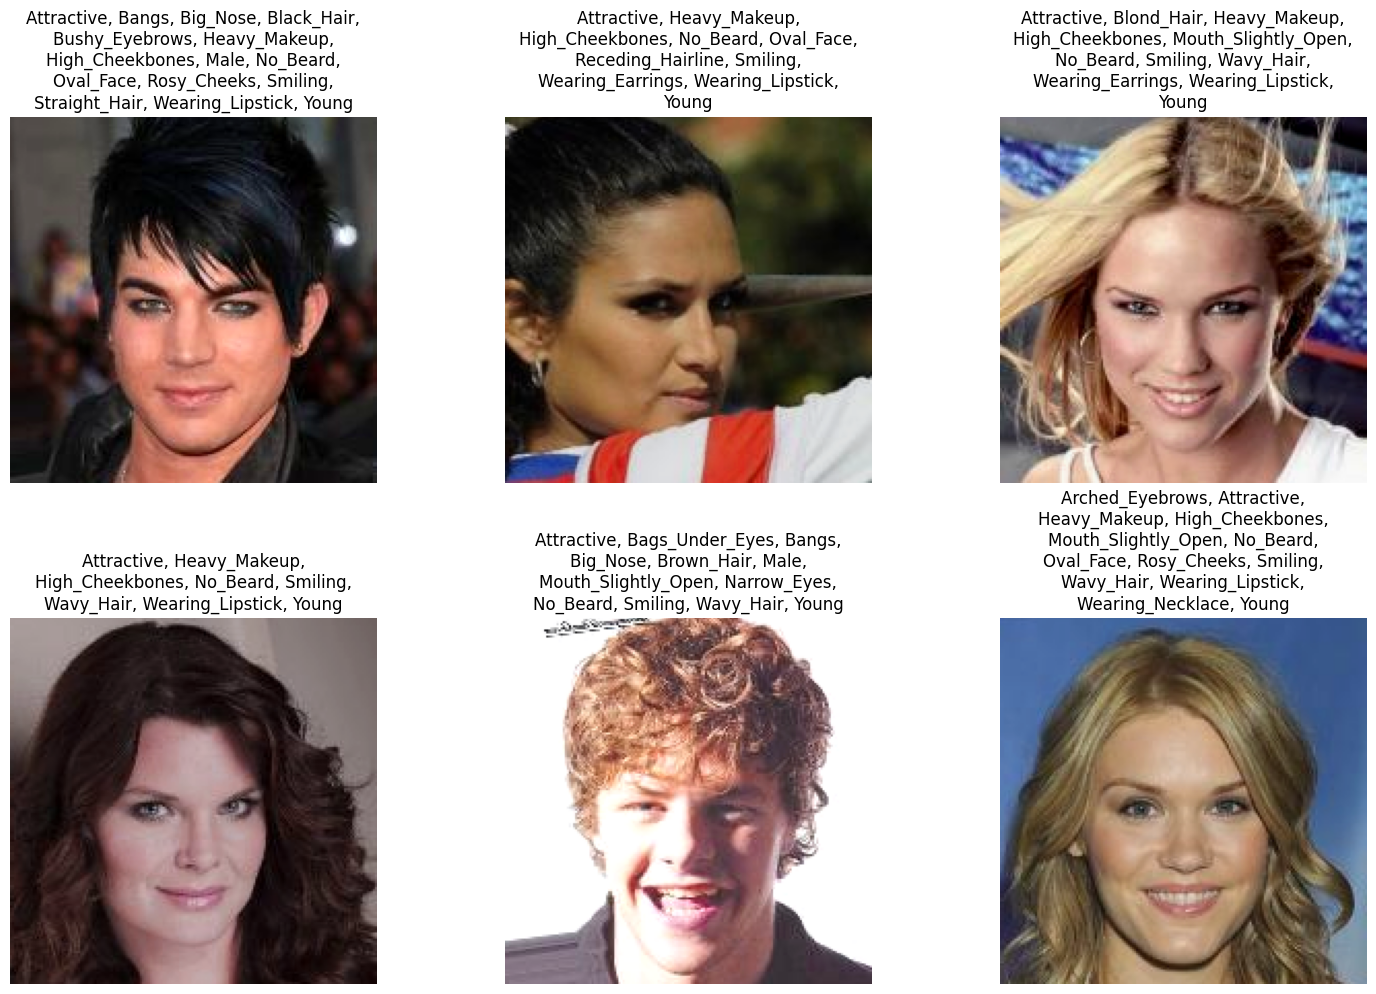
\includegraphics[width=0.5\textwidth]{DatasetSample.png}
  \centering
  \caption{Sample images from the CelebA dataset after preprocessing and augmentation.}
  \centering
  \end{wrapfigure}

For augmentation I have utilized the PyTorch's transformation library's second version, providing a way to easily add common augmentation techniques.

I applied the ColorJitter transformation to introduce controlled variations in brightness, contrast, saturation, and hue.
Specifically, I set the parameters to adjust brightness, contrast, and saturation by a maximum of 0.1, while allowing for a hue shift of up to 0.05.
This augmentation strategy diversifies the dataset by simulating real-world variations in lighting conditions and color appearances, thereby enhancing the model's resilience to such variations during inference.
Random Horizontal Flip to further enrich the dataset and promote model robustness, we incorporated random horizontal flipping. This simple yet effective transformation horizontally mirrors the images with a 50\% probability during training.
By introducing variations in facial orientations, this augmentation technique not only expands the dataset size but also encourages the model to learn invariant features, improving its ability to generalize across diverse facial poses and orientations.

By implementing these preprocessing and augmentation techniques, I optimized the dataset for training the model, fostering improved performance, generalization, and resilience to real-world variations.

\subsection{Model architecture}
\label{sec:subsection_model_architecture}

The foundation of our facial attribution recognition model is built upon the EfficientFormerV2 backbone, because of its efficiency and effectiveness in processing visual data it makes it capable for efficient attribute recognition.
Complementing this backbone architecture, our model employs multiple Feedforward Neural Network (FFN) heads to facilitate multi-task learning, inspired by \citet{DBLP:journals/corr/HandC16}, allowing for the simultaneous prediction of various facial attributes.
This approach is enhanced by the hierarchical structure of the FFN heads, inspired by \citet{DBLP:journals/corr/HanJSC17}, which are strategically grouped based on distinctive facial regions, enabling targeted feature extraction and attribute prediction.
These heads are strategically grouped based on distinctive facial regions, enabling targeted feature extraction and attribute prediction.

The EfficientFormerV2 backbone serves as the core of our model architecture, leveraging the advantages of transformer-based architectures for visual processing tasks.
Renowned for its computational efficiency and scalability, EfficientFormerV2 efficiently captures intricate spatial dependencies within input images, facilitating superior feature representation and extraction.

Our model incorporates seven FFN heads, each specializing in predicting attributes associated with specific facial regions (examples in parantheses):

\begin{itemize}
  \item 9 Whole Face attributes (Attractive, Male, Smiling, Young)
  \item 10 Hair related attributes (Bald, Bangs, Blond Hair)
  \item 5 Eye region related attributes (Eyeglasses, Narrow Eyes, Arched Eyebrows)
  \item 2 Nose related attributes (Big Nose, Pointy Nose)
  \item 9 attributes in the Lips and Chin area (Big Lips, Mustache, No Beard)
  \item 3 attributes in the Cheeks and Ear area (High Cheekbones, Rosy Cheeks)
  \item 2 Neck region attributes (Wearing Necklace, Wearing Necktie)
\end{itemize}

Each FFN head comprises multiple layers designed to extract and process features relevant to the corresponding facial region.
The architecture of each head follows a consistent pattern:

\begin{figure}[h]
  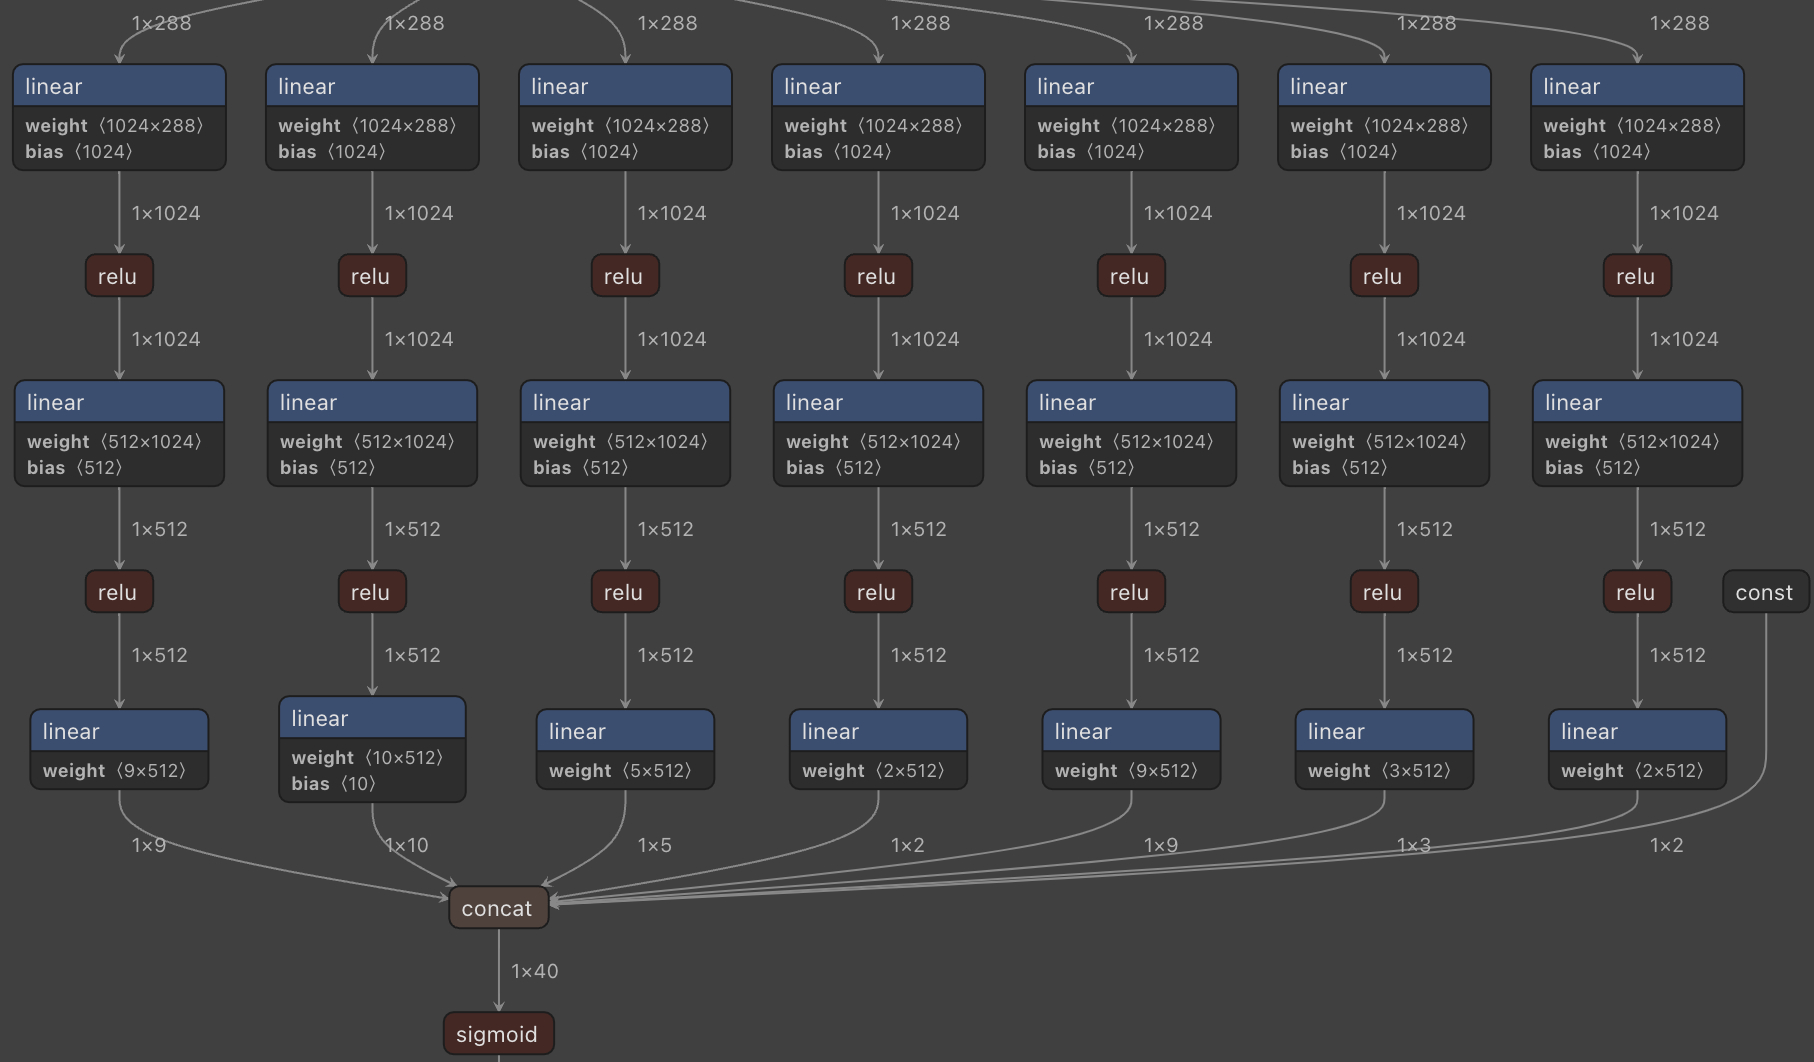
\includegraphics[width=\textwidth]{ModelHead.png}
  \centering
  \caption{The seven FFN heads visualized.}
  \centering
  \end{figure}

First Layer (1024 Neurons): The initial layer of each FFN head consists of 1024 neurons, serving as the primary feature extractor.
This layer processes input features from the EfficientFormerV2 backbone, capturing region-specific information essential for attribute prediction.

ReLU Activation Layer: Following the first layer, a Rectified Linear Unit (ReLU) \citet{DBLP:journals/corr/abs-1803-08375} activation function is applied to introduce non-linearity into the model.
This activation layer enhances the model's capacity to learn complex feature representations, enabling more expressive attribute predictions.
The ReLU activation function is chosen for its simplicity and efficiency in promoting model convergence and performance.

Second Layer (512 Neurons): Subsequently, another fully connected layer comprising 512 neurons is employed to further refine the extracted features.
This layer facilitates hierarchical feature abstraction, enabling the model to capture increasingly abstract representations of the input data.
Another ReLU layer follows this layer.

Concatenation: The outputs of the second layer from each FFN head are concatenated into a unified feature vector, consolidating the extracted features from all facial regions.

Sigmoid Activation: Finally, a sigmoid activation function is applied to the concatenated feature vector to perform binary classification for attribute prediction.
The sigmoid function produces probabilities indicating the likelihood of each attribute's presence, enabling the model to make informed predictions based on the learned features.

By adopting this multi-head FFN architecture, our model effectively leverages the hierarchical structure of facial attributes, enabling precise and comprehensive attribute prediction across diverse facial regions.
This architecture promotes holistic understanding of facial characteristics while accommodating the unique attributes associated with each region, thereby enhancing the model's performance and versatility in facial attribution recognition tasks.

In total the model has 15,608,472 trainable with 12.6 million parameters in the EfficientFormerV2 backbone and the remaining parameters in the FFN heads.

\subsection{Output transformation \& hyperparameters}
\label{sec:subsection_output_transformation}

Upon generating predictions using our multi-head FFN architecture, the model's output must be transformed to align with the labels in the dataset.
Given the introduction of regional grouping for attribute prediction, for further details please refer to section \ref{sec:subsection_model_architecture}, the order of labels in the model's output may differ from that of the dataset labels.
To facilitate accurate comparison, a transformation process is employed to reorder the model outputs accordingly.
Please note that that the transformation process is not included within the model as it is unnecessary overhead during inference, but rather applied post-prediction, during training and evaluation, to ensure consistency with the dataset labels.

On the figure below the dataset's label order is shown as ATTRIBUTES and the model's output order is shown as NEW\_ATTRIBUTES.

\begin{figure}[h]
  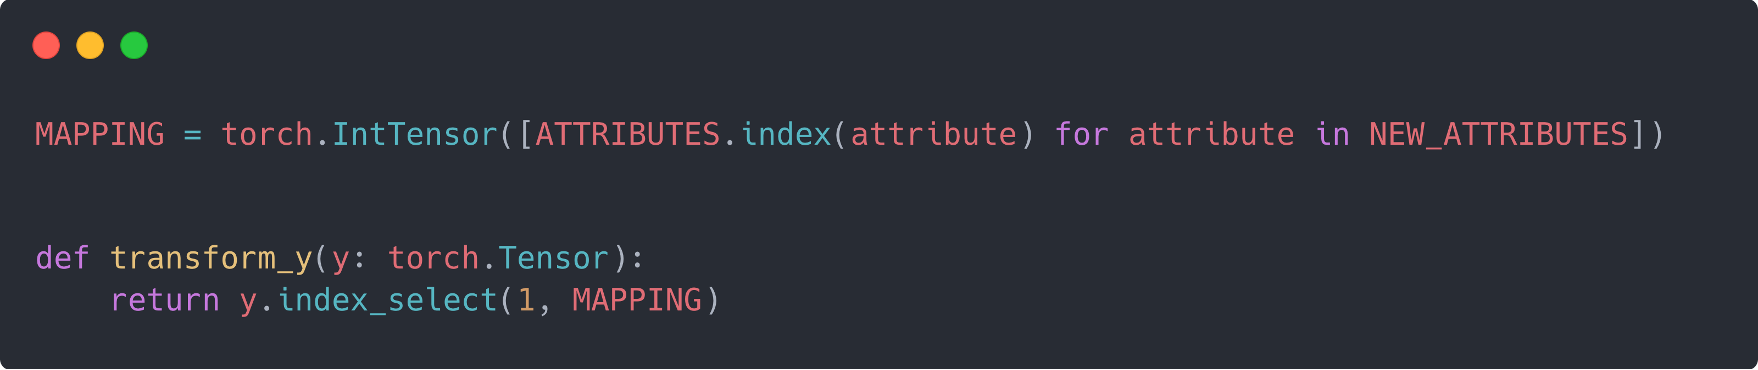
\includegraphics[width=\textwidth]{OutputTransformation.png}
  \centering
  \caption{Output transformation.}
  \centering
\end{figure}

During experimentation, the impact of various hyperparameters on model performance, including the configuration of the EfficientFormer V2 backbone, have been tested.

Firstly I investigated the effect of switching between the various predefined configurations of the EfficientFormer V2 architecture.
Despite initial expectations, transitioning from the S2 preset to a larger configuration (L2) did not yield improvements in model performance.
Moreover, this modification significantly extended the training time and memory requirements, impeding overall training efficiency without commensurate gains in predictive accuracy.

Secondly the hyperparameters of the Two-Layer FFN have been investigated.
The architecture of the FFN heads within my model comprises two fully connected layers, with 1024 and 512 neurons, respectively.
Throughout experimentation, I explored variations in the width and depth of these FFN layers to ascertain their impact on model performance.
Contrary to expectations, widening the FFN layers beyond the specified configuration did not yield appreciable enhancements in predictive accuracy.
Additionally, attempts to improve model generalization through the incorporation of Dropout layers proved ineffective, as they only served to prolong convergence without yielding tangible improvements in performance.

Through experimentation and hyperparameter tuning, I optimized the model architecture and hyperparameters to strike a balance between predictive accuracy and training efficiency.
The selected configuration reflects my efforts to maximize model performance while mitigating the risk of overfitting and training slowdowns.

\subsection{Training}
\label{sec:subsection_training}

During the training phase, the model utilizes binary cross-entropy loss as the objective function to quantify the disparity between predicted attribute probabilities and ground truth labels.
This loss function is particularly well-suited for binary classification tasks, such as facial attribute recognition, where each attribute is treated as a binary prediction task (presence or absence).

To optimize the model parameters and minimize the computed loss, the AdamW optimizer \citet{DBLP:journals/corr/abs-1711-05101} is used.
AdamW extends the Adam optimizer by incorporating weight decay regularization, thereby effectively preventing overfitting and enhancing model generalization.
This optimizer's adaptive learning rate mechanism enables efficient convergence and robust performance across diverse datasets and architectures.

To strike a balance between training efficiency and memory utilization, a batch size of 64 is used.
The value 64 is chosen as this is the highest batch size that can be accommodated within the available memory constraints, ensuring optimal hardware utilization during training.
By processing data in batches, parallelism is utilized to accelerate training iterations while ensuring optimal memory usage within the available hardware constraints.

I trained the model for 3 epochs on a single NVIDIA RTX 2070 SUPER GPU (8GB VRAM).
The choice of 3 epochs is based on empirical observations during training, where the model's performance plateaued after the third epoch.
Training takes approximately 30 minutes to complete, with each epoch lasting around 10 minutes.

\subsection{Results}
\label{sec:subsection_results}

The proposed facial attribution recognition model demonstrates promising performance on the test dataset, achieving an accuracy of 90.9\% with an average loss of 0.202585.
This performance metric highlights the model's proficiency in correctly identifying facial attributes from input images.

Additionally, the model exhibits a recall rate of 73.0\%, indicating its ability to effectively capture true positive instances among all actual positive cases.

Furthermore, the specificity of our model stands at 96.3\%, underscoring its capability to correctly identify negative instances among all actual negative cases.

Comparison with Existing Models:

My model approaches state-of-the-art performance in facial attribute recognition, showcasing competitive accuracy while offering notable advantages in training speed, inference speed, and model size.
Specifically, the model achieves an accuracy of 90.9\%, only marginally lagging behind the performance of the model presented in the TransFA paper \citet{liu2022transfa}, which reported an accuracy of 91.9\%.
However, my model outperforms TransFA in terms of training speed, inference speed, and model size as that uses the Swin Transformer architecture, which is inefficient compared to the EfficientFormerV2 architecture.

The DMM-CNN model by \citet{DBLP:journals/corr/abs-2002-03683} includes the parameter count and accuracy of their model, making it suitable for comparison.
Their model used 360 million parameters compared to just 15.6 million in my model, while achieving an accuracy of 91.7\%.

While there are no specific numbers reported for the specifics of the TransFA architecture regarding parameter count, training and inference speed,
I suspect they are using the base Swin Transformer architecture as their paper reports using 12 Swin Transformer Layers, making just the backbone of their model 121 million parameters.
Additionally their FFN heads use double the neurons in the first layer, making their head also use more parameters than mine.

\begin{wrapfigure}{l}{0.5\textwidth}
  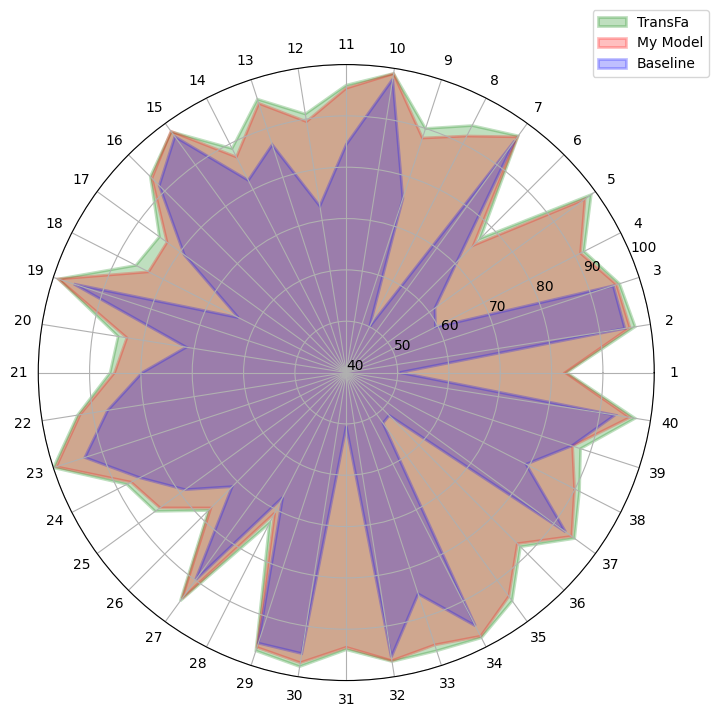
\includegraphics[width=0.5\textwidth]{radarplot.png}
  \centering
  \caption[Radar plot]{Radar plot per attribute performance visualization\footnotemark}
  \centering
\end{wrapfigure}

\footnotetext{
  The attributes are as follows:
  Attractive, Blurry, Chubby, Heavy Makeup, Male, Oval Face, Pale Skin, Smiling, Young
  Bald, Bangs, Black Hair, Blond Hair, Brown Hair, Gray Hair, Receding Hairline, Straight Hair, Wavy Hair, Wearing Hat
  Arched Eyebrows, Bags Under Eyes, Bushy Eyebrows, Eyeglasses, Narrow Eyes
  Big Nose, Pointy Nose,
  5 o'Clock Shadow, Big Lips, Double Chin, Goatee, Mouth Slightly Open, Mustache, No Beard, Sideburns, Wearing Lipstick
  High Cheekbones, Rosy Cheeks, Wearing Earrings
  Wearing Necklace, Wearing Necktie
}

In the radar plot on the left the performance of the model is visualized compared to the TransFA model.
A Baseline performance is calculated using the distribution of attributes in the dataset, if the probability of an attribute occuring is less than 0.5 it is subtracted from 1, otherwise it is left as is.
This subtraction is done to account for the imbalance in the dataset, as the model could achieve a high accuracy by just predicting the most common attributes.

The results of my study hold significant implications for the field of facial attribute recognition and related applications.
Despite slightly trailing behind the state-of-the-art models in accuracy, my model offers substantial improvements in terms of efficiency and resource utilization.
The enhanced training speed, inference speed, and reduced model size make my approach particularly appealing for real-world deployment in scenarios where computational resources are limited or efficiency is paramount.

In conclusion, the proposed facial attribution recognition model demonstrates competitive performance in accurately identifying facial attributes from input images.
While achieving a commendable accuracy of 90.9\%, my model distinguishes itself through its efficiency gains in training and inference, as well as its compact model size.
These findings underscore the potential of my approach to address the practical challenges associated with facial attribute recognition, paving the way for widespread adoption in various resource constrained applications.

\subsection{iOS Demo Application}
\label{sec:subsection_ios_demo}

To demonstrate the real-time capability of my facial attribution recognition model, I developed an intuitive iOS demo application using Swift and SwiftUI.
This application leverages the power of Core ML to deploy my PyTorch-based model directly onto iOS devices, enabling real-time inference on live camera feeds.

The first step in developing the iOS application involved converting the PyTorch model into a Core ML model using the CoreMLTools library.
This conversion process facilitated seamless integration of my model into the iOS ecosystem, allowing for efficient execution on Apple's hardware platforms.
CoreMLTools performs optimizations tailored for inference purposes, ensuring optimal performance and resource utilization on iOS devices.
CoreMLTools utilizes the following optimizations:


In the API there are common passes and cleanup passes defined.
For the purpose of this study only high-level, model related optimizations are listed.
Quantization is used to convert the model to 16-bit floating point numbers, reducing the model size and improving inference speed.
Layer fusion involves combining multiple operations or layers within the model into a single operation or layer, reducing the overall workload and improving efficiency.
During conversion padding optimizations ensure efficient convolutions by optimizing padding operations.
Dead code elimination removes unnecessary operations or layers from the model, reducing computational overhead and improving inference speed.
Transpose optimization rearranges data in the model to improve memory access patterns and reduce latency.

The converted Core ML model exhibited remarkable efficiency, achieving inference speeds as low as 1.18 milliseconds on high-end devices such as the iPhone 14 Pro Max.
After the conversion process I reran the model on the CelebA dataset to ensure that the conversion process did not affect the model's performance.
The model miraculously slightly improved its accuracy, achieving a score of 91\% on the test dataset, demonstrating the robustness and reliability of the Core ML conversion process.
The accuracy improvement can be attributed to the quantization process which can sometimes improve the model's performance by rounding off the weights and biases to the nearest 16-bit floating point number in a way that improves the model's performance.
Crucially, the model leveraged the device's neural engine for each calculation, harnessing specialized hardware acceleration to expedite inference tasks while conserving battery life.

\begin{figure}[h]
  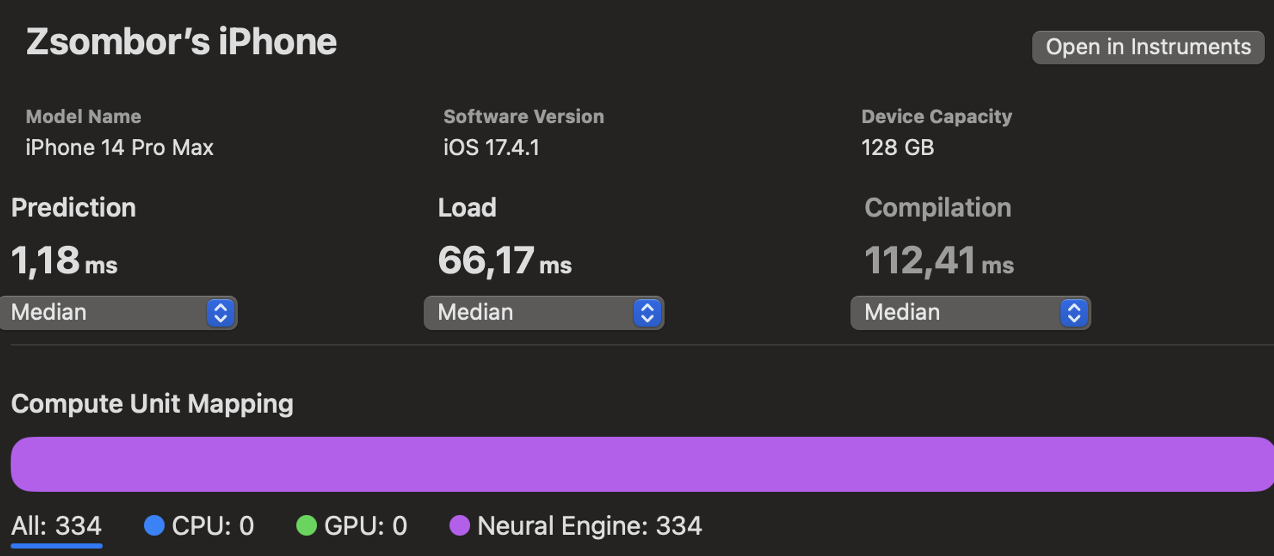
\includegraphics[width=\textwidth]{iOSInference.png}
  \centering
  \caption{iOS inference benchmark.}
  \centering
\end{figure}

\begin{wrapfigure}{r}{0.4\textwidth}
  
\includegraphics[width=0.4\textwidth]{iOSapp.jpeg}
  \centering
  \caption{iOS demo application interface.}
  \centering
\end{wrapfigure}

The iOS demo application features a user-friendly interface designed using SwiftUI, Apple's declarative framework for building user interfaces.
Upon launching the application, users are presented with a simple yet engaging interface, showcasing a circular frame in the center of the screen.
As users position their head within the designated circular frame, the application initiates real-time attribute recognition by capturing frames from the device's camera and passing them through the Core ML model.
The model analyzes each frame and identifies facial attributes deemed to be present, providing instant feedback on the bottom of the screen.
By doulbe tapping on the screen, users may stop the camera feed and model inference, allowing them to view the detected attributes in detail.
Doulbe tapping again resumes the camera feed and model inference.

Thanks to the low inference speed and efficient hardware utilization of the Core ML model, the iOS demo application delivers seamless performance with no dropped frames.
Users can experience smooth and uninterrupted attribute recognition.

My iOS demo application showcases the practical implications of a real-time facial attribution recognition model, extending its capabilities to mobile platforms and empowering users with real-time attribute recognition on their iOS devices.
By harnessing the power of Core ML and SwiftUI, I offer an intuitive and efficient solution for facial attribute analysis, opening doors to resource constrained applications in fields such as digital health and personalization.

\clearpage
\subsection{Summary}
\label{sec:summary}

During my project laboratory I researched state-of-the-art approaches in the field of facial attribute recognition, identified key challenges, and proposed novel solutions to enhance model efficiency while maintaining performance.
The study begins by reviewing earlier approaches to facial attribute recognition using deep learning, highlighting the contributions of convolutional neural networks (CNNs) and multi-task learning frameworks.

Moving forward, the paper discusses recent advancements in transformer-based architectures, such as the Vision Transformer (ViT) and Swin Transformer, in computer vision tasks and their limited application to facial attribute recognition.
It then delves into the development of TransFa, a transformer-based model utilizing the Swin Transformer architecture, which achieves state-of-the-art performance on the CelebA dataset.

The study addresses the computational complexity challenge inherent in transformer architectures by introducing the EfficientFormerV2, a lightweight transformer model optimized for efficient deployment on resource-constrained devices, particularly mobile devices.
In my approach I leverage the EfficientFormerV2 backbone to develop a facial attribute recognition model that excels in real-time performance, efficiency, and accuracy.

Furthermore, the paper provides a detailed overview of my use of data augmentation for training, enhancing dataset robustness and model performance.
It then describes the model architecture, which incorporates the EfficientFormerV2 backbone and multiple Feedforward Neural Network (FFN) heads for multi-task learning.

The study also discusses output transformation and hyperparameters optimization, outlining the choice of objective function, optimizer, batch size, and training epochs.
The model's performance is evaluated against state-of-the-art approaches in facial attribute recognition, highlighting its competitive accuracy, while signifanctly increasing training speed, inference speed, and decreasing model size.

In conclusion, the paper presents an intuitive iOS demo application showcasing real-time attribute recognition using the developed facial attribute recognition model.
Leveraging Core ML and SwiftUI, the application delivers seamless performance on iOS devices, demonstrating the practical implications of transformer-based models in real-world scenarios.

\newpage
%==================================================================
\section{References}
\label{sec:references}

\bibliographystyle{unsrtnat}
\bibliography{references}  %%% Uncomment this line and comment out the ``thebibliography'' section below to use the external .bib file (using bibtex) .

%\subsection{Attached documents}
%\label{sec:attached_documents}

%Source code etc.

\end{document} 

%%% Local Variables: 
%%% mode: latex 
%%% TeX-master: t 
%%% End:

